\documentclass[14pt,aspectratio=1610]{beamer}

\usepackage[brazil]{babel}
\usepackage[utf8]{inputenc}
%\UseRawInputEncoding
\usepackage[T1]{fontenc}
\usepackage{Sweave}
\usepackage{animate}
\usepackage{amsbsy}
\usepackage{amsfonts}
\usepackage{amsmath}
\usepackage{amssymb}
\usepackage{amsthm}
\usepackage[toc,page,title,titletoc]{appendix}
\usepackage[fixlanguage]{babelbib}
%\usepackage[pdftex]{color}
\usepackage{dsfont}
\usepackage{esvect}
\usepackage[labelfont=bf]{caption}
\usepackage{float}
\usepackage[Glenn]{fncychap}%Sonny %Conny %Lenny %Glenn %Renje %Bjarne %Bjornstrup
%\usepackage{geometry, calc, color, setspace}%
%\geometry{a4paper, headsep=1.0cm, footskip=1cm, lmargin=3cm, rmargin=2cm, tmargin=3cm, bmargin=2cm}
\usepackage{graphicx}
\usepackage{indentfirst}%Para indentar os parágrafos automáticamente
\usepackage{lipsum}
\usepackage{longtable}
\usepackage{mathtools}
\usepackage{listings}%Inserir codigo do R no latex
\usepackage{multirow}
\usepackage{multicol}
\usepackage{natbib}
\bibliographystyle{abbrvnat3}
\usepackage[figuresright]{rotating}
\usepackage{spalign}
%\usepackage{pgfpages}
\usepackage{pgfplots}
\usepackage{tikz}
\usepackage{color, colortbl}
\usepackage{ragged2e}%para justificar o texto dentro de algum ambiente
\definecolor{Gray}{gray}{0.9}
\definecolor{LightCyan}{rgb}{0.88,1,1}


\usepackage[all]{xy}
\usepackage{hyperref,bookmark}
\hypersetup{
  colorlinks=true,
  linkcolor=blue,
  citecolor=red,
  filecolor=blue,
  urlcolor=blue,
}

\usetheme{AnnArbor}
%\usecolortheme[RGB={19,20,80}]{structure}
\definecolor{seagull}{rgb}{.125,.5,.25}
%\setbeamertemplate{footline}[frame number]
%\setbeamertemplate{footline}[text line]{%
%  \parbox{\linewidth}{\vspace*{-8pt}\hfill\date{}\hfill\insertshortauthor\hfill\insertpagenumber}}
\beamertemplatenavigationsymbolsempty
\renewcommand{\vec}[1]{\mbox{\boldmath$#1$}}
\newtheorem{Teorema}{Teorema}
\newtheorem{Proposicao}{Proposição}
\newtheorem{Definicao}{Definição}
\newtheorem{Corolario}{Corolário}
\newtheorem{Demonstracao}{Demonstração}
\newcommand{\bx}{\ensuremath{\bar{x}}}
\newcommand{\Ho}{\ensuremath{H_{0}}}
\newcommand{\Hi}{\ensuremath{H_{1}}}


\apptocmd{\frame}{}{\justifying}{} % Allow optional arguments after frame.

\title{MAF 261 - Estatística Experimental}
\author{Prof. Fernando de Souza Bastos}
\institute{Instituto de Ciências Exatas e Tecnológicas\texorpdfstring{\\ Universidade Federal de Viçosa}{}\texorpdfstring{\\ Campus UFV - Florestal}{}}
\date{09/08/2018}
\newcommand\mytext{Aula sobre Distribuição Normal}
\newcommand\mytextt{Fernando de Souza Bastos}
\makeatletter
\setbeamertemplate{footline}
{
  \leavevmode%
  \hbox{%
  \begin{beamercolorbox}[wd=.333333\paperwidth,ht=2.25ex,dp=1ex,center]{author in head/foot}%
    \usebeamerfont{author in head/foot}\mytext
  \end{beamercolorbox}%
  \begin{beamercolorbox}[wd=.333333\paperwidth,ht=2.25ex,dp=1ex,center]{title in head/foot}%
    \usebeamerfont{title in head/foot}\mytextt
  \end{beamercolorbox}%
  \begin{beamercolorbox}[wd=.333333\paperwidth,ht=2.25ex,dp=1ex,right]{date in head/foot}%
    \usebeamerfont{date in head/foot}\insertshortdate{}\hspace*{2em}
    \insertframenumber{} / \inserttotalframenumber\hspace*{2ex} 
  \end{beamercolorbox}}%
  \vskip0pt%
}
\makeatother


\providecommand{\arcsin}{} \renewcommand{\arcsin}{\hspace{2pt}\textrm{arcsen}}
\providecommand{\sin}{} \renewcommand{\sin}{\hspace{2pt}\textrm{sen}}
%\newtheorem{Teorema}{Teorema}
%\newtheorem{Proposicao}{Proposição}
%\newtheorem{Definicao}{Definição}
%\newtheorem{Corolario}{Corolário}
%\newtheorem{Demonstracao}{Demonstração}

% Layout da pagina
\hypersetup{pdfpagelayout=SinglePage}
\begin{document}
\Sconcordance{concordance:normal_distribution.tex:normal_distribution.Rnw:%
1 130 1 1 16 1 4 84 1 1 23 1 4 246 1 1 3 2 0 1 2 1 0 1 1 4 0 1 3 5 1 1 %
15 14 0 1 1 4 0 1 3 5 1 1 3 2 0 4 1 1 3 2 0 1 1 4 0 1 3 17 1 1 3 26 0 1 %
3 10 1 1 3 26 0 1 3 5 1}


\pgfmathdeclarefunction{gauss}{2}{%
  \pgfmathparse{1/(#2*sqrt(2*pi))*exp(-((x-#1)^2)/(2*#2^2))}%
}

\frame{\titlepage}

\begin{frame}{}
\frametitle{\bf Sumário}
\tableofcontents
\end{frame}

\section{Introdução}
\begin{frame}[fragile]{}
\frametitle{Introdução}
Considere o peso, em kg, de 2000 jovens selecionados ao acaso entre todos os alunos da UFV, cujo histograma é apresentado:
\vspace{-1cm}
\begin{center}
\setkeys{Gin}{width=0.5\linewidth}
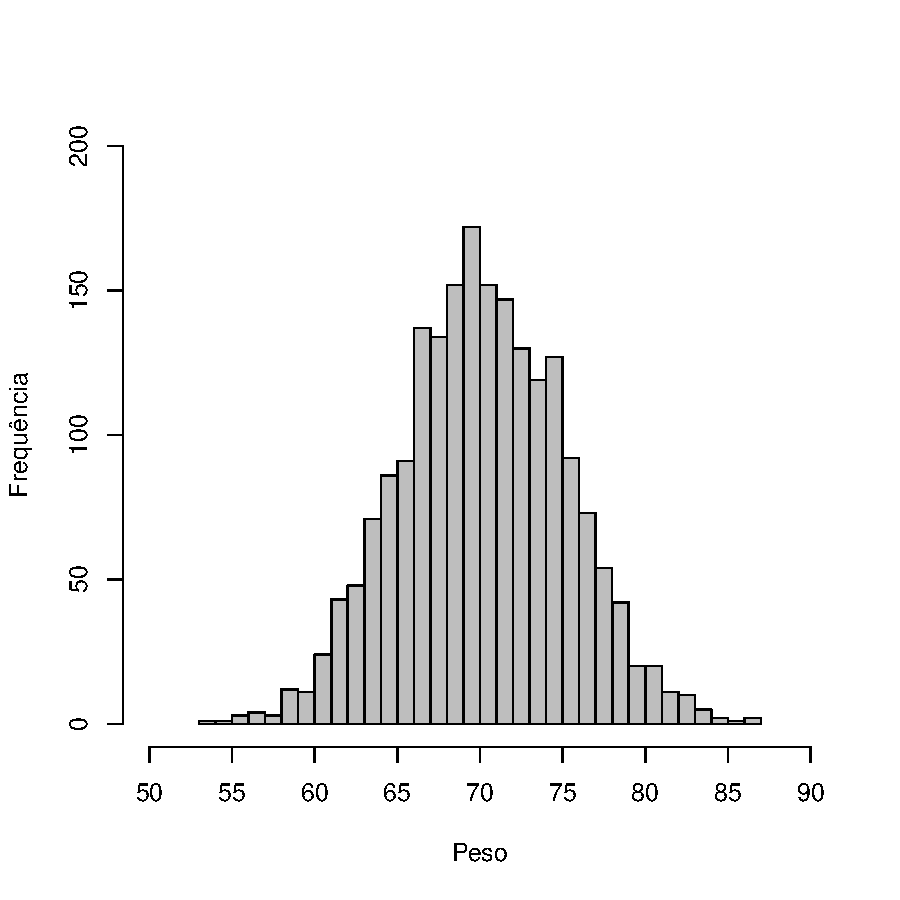
\includegraphics{normal_distribution-001}
\end{center}
\end{frame}

\begin{frame}{}
\frametitle{Introdução}
\begin{block}{}
\justifying
A análise do histograma indica que:
\begin{itemize}
\item a distribuição dos valores é aproximadamente simétrica em torno de 70 kg;
\item a maioria dos valores encontra-se no intervalo (60;80);
\item existe uma pequena proporção de valores abaixo de 55kg e acima de 85kg.
\end{itemize}
\end{block}
\end{frame}

\begin{frame}{}
\frametitle{Introdução}
\begin{block}{}
\justifying
A distribuição normal (algumas vezes chamada de distribuição de Gauss) é a distribuição contínua mais habitualmente utilizada no campo da estatística. Ela é de vital importância na estatística, por três razões principais:
\begin{itemize}
\item Inúmeras variáveis contínuas comuns no mundo dos negócios possuem distribuições que se assemelham estreitamente à distribuição normal. \pause
\item A distribuição normal pode ser utilizada para fazer aproximações para várias distribuições de probabilidades discretas.\pause
\item A distribuição normal proporciona a base para a inferência estatística clássica, em razão de sua relação com o Teorema do Limite Central.
\end{itemize}
\end{block}
\end{frame}

\begin{frame}{}
\frametitle{Introdução}
\begin{block}{}
\justifying
A distribuição normal é representada pelo clássico formato de sino. Na distribuição normal, você pode calcular a probabilidade de que venham a ocorrer valores dentro dos limites de determinadas amplitudes ou intervalos. No entanto, uma vez que a probabilidade para variáveis contínuas é mensurada como uma área abaixo da curva, a probabilidade exata de um valor específico, a partir de uma distribuição contínua tal como a distribuição normal, é zero. 
\end{block}
\end{frame}

\begin{frame}{}
\frametitle{Introdução}
\begin{block}{}
\justifying
A distribuição normal possui várias propriedades teóricas importantes:
\begin{itemize}
\item Ela é simétrica, sua média aritmética, sua mediana e sua moda são, consequentemente, iguais.
\item Em sua aparência, ela tem o formato de um sino.
\item Sua amplitude interquartil é igual a 1,349 desvio-padrão. Consequentemente, os 50\% valores centrais estão contidos dentro dos limites de um intervalo que tem como valores fronteiriços dois terços de um desvio-padrão abaixo da média aritmética e dois terços de um desvio-padrão acima da média aritmética.
\item Possui uma amplitude infinita $(\infty\leq X\leq \infty).$
\end{itemize}
\end{block}
\end{frame}

\begin{frame}{}
\frametitle{}
%\vspace{-1cm}
\begin{figure}[H]
    \centering
    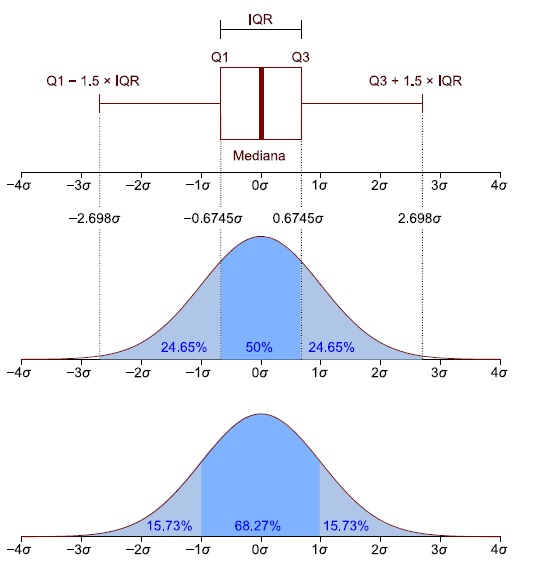
\includegraphics[height=0.6\textwidth, width=0.8\textwidth]{Amplitude_interquartil}
    %\caption{Legenda}
    %\label{figRotulo}
  \end{figure}
\end{frame}

\begin{frame}{}
\frametitle{Função Densidade para a probabilidade normal}
\begin{block}{}
\justifying
\begin{equation}
f(X)=\dfrac{1}{\sqrt{2\pi}\sigma}\exp{\Biggl[-\dfrac{(X-\mu)^{2}}{2\sigma^{2}}\Biggl]},\ X\in  \mathds{R},
\end{equation}
em que $\mu$ é a média aritimética e $\sigma$ é o desvio-padrão.
\end{block}
\end{frame}

\begin{frame}{}
\frametitle{Introdução}
\begin{block}{}
\justifying
Embora a Equação possa parecer complicada, as probabilidades da variável aleatória $X$ dependem somente de dois parâmetro, a média aritmética, $\mu$, e o desvio-padrão, $\sigma$. Todas as vezes que você determina valores específicos para $\mu$ e $\sigma$, é gerada uma distribuição de probabilidade normal diferente.
\end{block}
\end{frame}

\begin{frame}{}
\frametitle{}
\begin{center}
\setkeys{Gin}{width=0.65\linewidth}
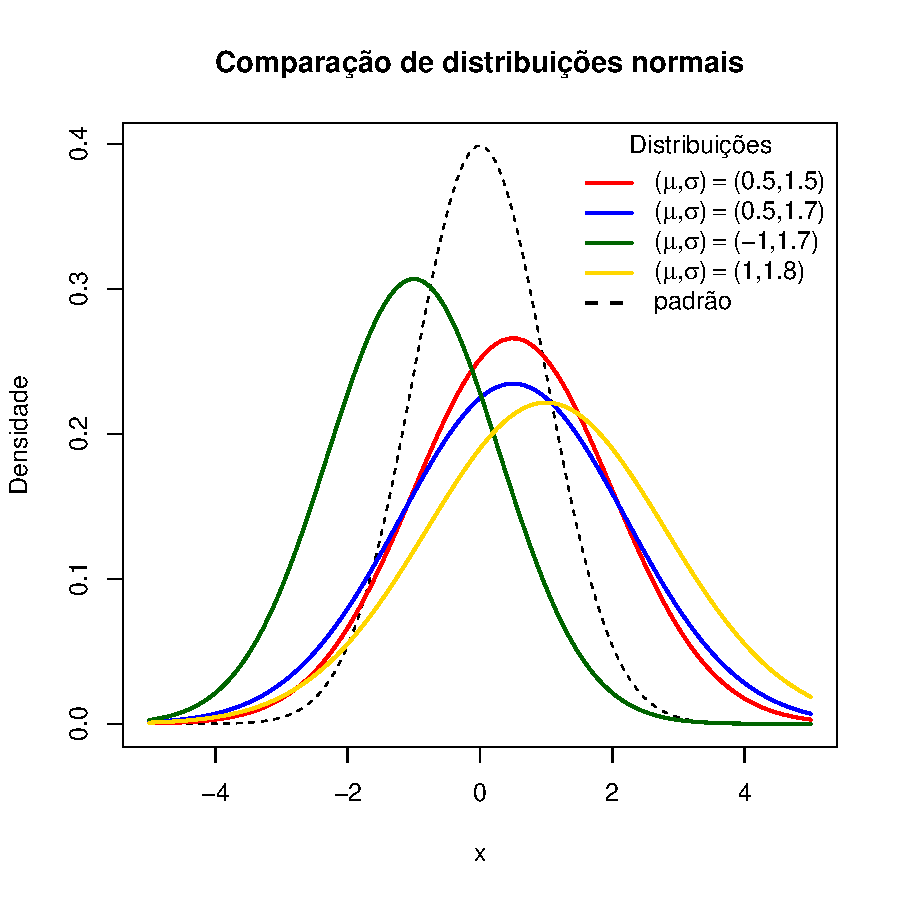
\includegraphics{normal_distribution-002}
\end{center}
\end{frame}

\begin{frame}{}
\begin{center}
\begin{tikzpicture}
\begin{axis}[
  xmin=-8,xmax=8,
  ymin=0,ymax=0.2,
  domain=-8:8, samples=100,
  axis lines=left, xlabel=$\bar{x}$, ylabel=Densidade de Probabilidade,
  %every axis y label/.style={at=(current axis.above origin),anchor=south},
  %every axis x label/.style={at=(current axis.right of origin),anchor=west},
  height=8cm, width=10cm,
  ticks=both,
  xtick={}, ytick=\empty,
  enlargelimits=false, axis on top, %clip=false, 
  %grid = major
  ]
  \addplot [very thick,cyan!50!black] {gauss(-2,2)};
  \node [right] at (axis cs: -7, .15) {$N(-2,\sigma^{2})$};
  \draw[very thick] (axis cs:-2,0) -- (axis cs:-2,0.2);
  \addplot [dashed,cyan!50!black] {gauss(2,2)};
  \node [right] at (axis cs: 4,.15) {$N(2,\sigma^{2})$};
  \draw[dashed] (axis cs:2,0) -- (axis cs:2,0.2);
\end{axis}
\end{tikzpicture}
\end{center}
\end{frame}

\begin{frame}{}
\frametitle{}
\begin{center}
\begin{tikzpicture}[
  declare function={
    normalpdf(\x,\mu,\sigma)=
    (2*3.1415*\sigma^2)^(-0.5)*exp(-(\x-\mu)^2/(2*\sigma^2));
  },
  hplot/.style={ycomb, mark=o, dashed}]

  \begin{axis}[
    width=12cm, height=6cm,
    samples=50,
    xlabel=$x$, ylabel=$f(x)$,
    xlabel style={at={(1,0)}, anchor=north west},
    ylabel style={rotate=-90, at={(0,1)}, anchor=south east},
    legend style={draw=none, fill=none},
    domain=-6:9,
    legend cell align=left,
    xmin=-7, xmax=11]

    \addplot [smooth, thick] {normalpdf(x,0,1)}
    node[pos=0.47, pin={right:$\mu=0,\sigma^2=1$}] {};
    \addplot [smooth, blue] {normalpdf(x,0,2)}
    node[pos=0.6, pin={45:$\mu=0,\sigma^2=2$}] {};
    \addplot [smooth, red] {normalpdf(x,-2,1)}
    node[pos=0.25, pin={[text centered, text width=8ex]
      200:$\mu=-1$, $\sigma^2=1$}] {};

    \addplot [hplot, samples at={0}] {normalpdf(x,0,1)};
    \addplot [hplot, samples at={0}, blue] {normalpdf(x,0,2)};
    \addplot [hplot, samples at={-2}, red] {normalpdf(x,-2,1)};

    % \node[anchor=north east] at (axis description cs: 0.975,  0.95)
    % {$f(x) = \dfrac{1}{\sqrt{2\pi\sigma^2}}\cdot 
    %   \exp\left\{-\frac{(x-\mu)^2}{2\sigma^2}\right\}$};

  \end{axis}
\end{tikzpicture}
\end{center}
\end{frame}

\begin{frame}{}
\frametitle{Cálculo de Probabilidades}
\begin{center}
\begin{tikzpicture}
\begin{axis}[
  xmin=-10,xmax=10,
  ymin=0,ymax=0.15,
  domain=-8:8, samples=100,
  axis y line*=left,
  y axis line style={draw opacity=0},
  axis x line=left, xlabel=$P(a\leq X\leq b)$, %ylabel=Densidade de Probabilidade,
  %every axis y label/.style={at=(current axis.above origin),anchor=south},
  %%every axis x label/.style={at=(current axis.right of origin),anchor=west},
  height=8cm, width=10cm,
  ticks=both,
  xtick=\empty, ytick=\empty,
  %enlargelimits=false, axis on top, %clip=false, 
  %%grid = major
  ]
  \addplot [fill=cyan!20, draw=none, domain=-1:2] {gauss(0,3)} \closedcycle;
  \addplot [very thick,cyan!50!black] {gauss(0,3)};
  \draw[very thick] (axis cs:-1,0) -- (axis cs:-1,0.125);
  \draw[very thick] (axis cs: 2,0) -- (axis cs: 2,0.107);
  \draw[dashed] (axis cs:0,0) -- (axis cs:0,0.131);
  \end{axis}
\end{tikzpicture}
\end{center}
\end{frame}

\begin{frame}{}
\frametitle{}
\begin{block}{}
\justifying
Se $X\sim N(\mu,\sigma^{2})$ então $Z=\dfrac{X-\mu}{\sigma}\sim N(0,1).$
\end{block}
\begin{block}{}
\justifying
A variável $Z\sim N(0,1)$ denomina-se normal padrão ou normal reduzida. Notemos que:

$$P(a\leq X\leq b)=P\Biggl(\dfrac{a-\mu}{\sigma}\leq\dfrac{X-\mu}{\sigma}\leq\dfrac{b-\mu}{\sigma}\Biggl)$$

e, dado a variável $Z\sim N(0,1),$ podemos obter $X\sim N(\mu,\sigma^{2})$ através da transformação inversa:

$$X=\mu+Z\sigma$$

\end{block}
\end{frame}

\section{Uso da Tabela}
\begin{frame}{}
\frametitle{Exemplos}
\begin{block}{}
\justifying
Dado $Z\sim N(0,1),$ calcule $P(Z\leq 0.5)$
\end{block}
\begin{center}
\begin{tikzpicture}[scale=0.8]
\begin{axis}[
  xmin=-10,xmax=10,
  ymin=0,ymax=0.15,
  domain=-10:10, samples=100,
  axis y line*=left,
  y axis line style={draw opacity=0},
  axis x line=left, xlabel={$P(Z\leq 0)=0.5$}, %ylabel=Densidade de Probabilidade,
  %every axis y label/.style={at=(current axis.above origin),anchor=south},
  %%every axis x label/.style={at=(current axis.right of origin),anchor=west},
  height=8cm, width=10cm,
  ticks=both,
  xtick={0}, ytick=\empty,
  %enlargelimits=false, axis on top, %clip=false, 
  %%grid = major
  ]
  \addplot [fill=cyan!20, draw=none, domain=-10:0] {gauss(0,3)} \closedcycle;
  \addplot [very thick,cyan!50!black] {gauss(0,3)};
  %\draw[very thick] (axis cs:-1,0) -- (axis cs:-1,0.125);
  \draw[very thick] (axis cs: 0,0) -- (axis cs: 0,0.131);
  %\draw[dashed] (axis cs:0,0) -- (axis cs:0,0.131);
  \end{axis}
\end{tikzpicture}
\end{center}
\end{frame}

\begin{frame}{}
\begin{minipage}{.3\linewidth}
    \begin{align*}
        P(Z\leq 0.32)&=0.5+P(0\leq Z\leq 0.32)\\
        &=0.5+0.1255\\
        &=0.6255
    \end{align*}
\end{minipage}%
\hspace{-2cm}
\begin{minipage}{0.1\linewidth}
    \centering
    \begin{tikzpicture}
        \begin{axis}[
  xmin=-10,xmax=10,
  ymin=0,ymax=0.15,
  domain=-10:10, samples=100,
  axis y line*=left,
  y axis line style={draw opacity=0},
  axis x line=left, xlabel={$P(Z\leq 0)=0.6255$}, %ylabel=Densidade de Probabilidade,
  %every axis y label/.style={at=(current axis.above origin),anchor=south},
  %%every axis x label/.style={at=(current axis.right of origin),anchor=west},
  height=8cm, width=10cm,
  ticks=both,
  xtick={0}, ytick=\empty,
  %enlargelimits=false, axis on top, %clip=false, 
  %%grid = major
  ]
  \addplot [fill=cyan!20, draw=none, domain=-10:0.32] {gauss(0,3)} \closedcycle;
  \addplot [very thick,cyan!50!black] {gauss(0,3)};
  %\draw[very thick] (axis cs:-1,0) -- (axis cs:-1,0.125);
  \draw[very thick] (axis cs: 0.32,0) -- (axis cs: 0.32,0.132);
  %\draw[dashed] (axis cs:0,0) -- (axis cs:0,0.131);
  \end{axis}
    \end{tikzpicture}
\end{minipage}
\end{frame}

\begin{frame}{}
\frametitle{Calcule:}
\begin{enumerate}
\item $P(0<Z\leq 1.71)=?$
\item $P(1.32\leq Z \leq 1.79)=?$
\item $P(Z\geq 1.5)=?$
\item $P(Z\leq -1.3)=?$
\item $P(-1.5\leq Z\leq 1.5)=?$
\item $P(-1.32 < Z <0)=?$
\item $P(-2.3<Z\leq -1.49)=?$
\item $P(-1\leq Z \leq 2)=?$
\item $P(Z\leq z)=0.975,$ qual o valor de $z?$
\item $P(0< Z \leq z)=0.4975,$ qual o valor de $z?$
\item $P(Z\geq z)=0.3,$ qual o valor de $z?$
\item $P(Z\geq z)=0.975,$ qual o valor de $z?$
\end{enumerate}
\end{frame}

\begin{frame}{}
\begin{enumerate}
\item $P(0<Z\leq 1.71)=0.4564$
\item $P(1.32\leq Z \leq 1.79)=0.0567$
\item $P(Z\geq 1.5)=0.0668$
\item $P(Z\leq -1.3)=0.0968$
\item $P(-1.5\leq Z\leq 1.5)=0.8664$
\item $P(-1.32 < Z <0)=0.4066$
\item $P(-2.3<Z\leq -1.49)=0.0574$
\item $P(-1\leq Z \leq 2)=0.8186$
\item $P(Z\leq z)=0.975,$ o valor de $z$ é $1.96.$
\item $P(0< Z \leq z)=0.4975,$ o valor de $z$ é $2.81.$
\item $P(Z\geq z)=0.3,$ o valor de $z$ é $0.53.$
\item $P(Z\geq z)=0.975,$ o valor de $z$ é $-1.96.$
\end{enumerate}
\end{frame}

\begin{frame}{}
Seja $X\sim N(10,64).$ Calcule:
\begin{enumerate}
\item $P(6<X\leq 12)=?$
\item $k$ tal que $P(X\geq k)=0.05$
\item $k$ tal que $P(X\leq k)=0.025$
\item $P(Z\leq -1.3)=?$
\item $P(-1.5\leq Z\leq 1.5)=?$
\item $P(-1.32 < Z <0)=?$
\item $P(-2.3<Z\leq -1.49)=?$
\item $P(-1\leq Z \leq 2)=?$
\item $P(Z\leq z)=0.975,$ qual o valor de $z?$
\item $P(0< Z \leq z)=0.4975,$ qual o valor de $z?$
\item $P(Z\geq z)=0.3,$ qual o valor de $z?$
\item $P(Z\geq z)=0.975,$ qual o valor de $z?$
\end{enumerate}
\end{frame}

\begin{frame}[fragile]{}
\frametitle{}
\begin{block}{}
\begin{Schunk}
\begin{Sinput}
> #------------------------------------------------
> dir.create("exemplos")
> png(file="exemplos/qnorm%1d.png", width=500, 
+ height=250)
> par(mar=c(4,4,1,1))
> #------------------------------------------------
\end{Sinput}
\end{Schunk}
\end{block}
\end{frame}

\begin{frame}[fragile]{}
\frametitle{}
\begin{block}{}
\begin{Schunk}
\begin{Sinput}
> #-----------------------------------------------
> for(q in seq(0, 4,l=100)){
+   curve(dnorm(x, 0, 1), -5, 5, ylab="f(z)", xlab="z")
+   x <- seq(0, q, by=0.01)
+   fx <- dnorm(x, 0, 1)
+   polygon(c(x, rev(x)),
+           c(fx, rep(0, length(fx))),
+           col="gray90")
+   abline(v=0, lty=2)
+   Pr <- round(pnorm(q, 0, 1)-0.5, digits=3)
+   qq <- round(q, digits=3)
+   legend("topleft", bty="n", fill="gray90",
+          legend=substitute(P(0<~Z<=~q)==Pr, 
+                            list(q=qq, Pr=Pr)))}
> dev.off()
> #-----------------------------------------------
\end{Sinput}
\end{Schunk}
\end{block}
\end{frame}

\begin{frame}[fragile]{}
\frametitle{}
\begin{block}{}
\begin{Schunk}
\begin{Sinput}
> #-----------------------------------------------
> require(xtable)
> options(OutDec=",")
> q <- seq(0,3.99,by=0.01)
> p <- pnorm(q)-0.5
> m <- matrix(p, byrow=TRUE, ncol=10)
> rownames(m) <- gsub("\\.", ",", 
+                     formatC(seq(0,3.9,0.1),
+                             dig=1, format="f"))
> colnames(m) <- 0:9/100
> #-----------------------------------------------
\end{Sinput}
\end{Schunk}
\end{block}
\end{frame}

\begin{frame}[fragile]{}
\frametitle{}
\begin{block}{}
\begin{center}
\animategraphics[controls, loop, width=0.75\textwidth]{10}{exemplos/qnorm}{1}{100}
\end{center}
\end{block}
\end{frame}

\begin{frame}[fragile]{}
\frametitle{}
\begin{block}{}
\begin{center}
\small\addtolength{\tabcolsep}{-3pt}
{\footnotesize
% latex table generated in R 3.4.3 by xtable 1.8-2 package
% Mon Aug 13 21:35:26 2018
\begin{tabular}{rrrrrrrrrrr}
  \hline
 & 0 & 0,01 & 0,02 & 0,03 & 0,04 & 0,05 & 0,06 & 0,07 & 0,08 & 0,09 \\ 
  \hline
0,0 & 0,00000 & 0,00399 & 0,00798 & 0,01197 & 0,01595 & 0,01994 & 0,02392 & 0,02790 & 0,03188 & 0,03586 \\ 
  0,1 & 0,03983 & 0,04380 & 0,04776 & 0,05172 & 0,05567 & 0,05962 & 0,06356 & 0,06749 & 0,07142 & 0,07535 \\ 
  0,2 & 0,07926 & 0,08317 & 0,08706 & 0,09095 & 0,09483 & 0,09871 & 0,10257 & 0,10642 & 0,11026 & 0,11409 \\ 
  0,3 & 0,11791 & 0,12172 & 0,12552 & 0,12930 & 0,13307 & 0,13683 & 0,14058 & 0,14431 & 0,14803 & 0,15173 \\ 
  0,4 & 0,15542 & 0,15910 & 0,16276 & 0,16640 & 0,17003 & 0,17364 & 0,17724 & 0,18082 & 0,18439 & 0,18793 \\ 
  0,5 & 0,19146 & 0,19497 & 0,19847 & 0,20194 & 0,20540 & 0,20884 & 0,21226 & 0,21566 & 0,21904 & 0,22240 \\ 
  0,6 & 0,22575 & 0,22907 & 0,23237 & 0,23565 & 0,23891 & 0,24215 & 0,24537 & 0,24857 & 0,25175 & 0,25490 \\ 
  0,7 & 0,25804 & 0,26115 & 0,26424 & 0,26730 & 0,27035 & 0,27337 & 0,27637 & 0,27935 & 0,28230 & 0,28524 \\ 
  0,8 & 0,28814 & 0,29103 & 0,29389 & 0,29673 & 0,29955 & 0,30234 & 0,30511 & 0,30785 & 0,31057 & 0,31327 \\ 
  0,9 & 0,31594 & 0,31859 & 0,32121 & 0,32381 & 0,32639 & 0,32894 & 0,33147 & 0,33398 & 0,33646 & 0,33891 \\ 
  1,0 & 0,34134 & 0,34375 & 0,34614 & 0,34849 & 0,35083 & 0,35314 & 0,35543 & 0,35769 & 0,35993 & 0,36214 \\ 
  1,1 & 0,36433 & 0,36650 & 0,36864 & 0,37076 & 0,37286 & 0,37493 & 0,37698 & 0,37900 & 0,38100 & 0,38298 \\ 
  1,2 & 0,38493 & 0,38686 & 0,38877 & 0,39065 & 0,39251 & 0,39435 & 0,39617 & 0,39796 & 0,39973 & 0,40147 \\ 
  1,3 & 0,40320 & 0,40490 & 0,40658 & 0,40824 & 0,40988 & 0,41149 & 0,41309 & 0,41466 & 0,41621 & 0,41774 \\ 
  1,4 & 0,41924 & 0,42073 & 0,42220 & 0,42364 & 0,42507 & 0,42647 & 0,42785 & 0,42922 & 0,43056 & 0,43189 \\ 
  1,5 & 0,43319 & 0,43448 & 0,43574 & 0,43699 & 0,43822 & 0,43943 & 0,44062 & 0,44179 & 0,44295 & 0,44408 \\ 
  1,6 & 0,44520 & 0,44630 & 0,44738 & 0,44845 & 0,44950 & 0,45053 & 0,45154 & 0,45254 & 0,45352 & 0,45449 \\ 
  1,7 & 0,45543 & 0,45637 & 0,45728 & 0,45818 & 0,45907 & 0,45994 & 0,46080 & 0,46164 & 0,46246 & 0,46327 \\ 
  1,8 & 0,46407 & 0,46485 & 0,46562 & 0,46638 & 0,46712 & 0,46784 & 0,46856 & 0,46926 & 0,46995 & 0,47062 \\ 
  1,9 & 0,47128 & 0,47193 & 0,47257 & 0,47320 & 0,47381 & 0,47441 & 0,47500 & 0,47558 & 0,47615 & 0,47670 \\ 
   \hline
\end{tabular}}
\end{center}
\end{block}
\end{frame}

\begin{frame}[fragile]{}
\frametitle{}
\begin{block}{}
\begin{center}
\small\addtolength{\tabcolsep}{-3pt}
{\footnotesize
% latex table generated in R 3.4.3 by xtable 1.8-2 package
% Mon Aug 13 21:35:26 2018
\begin{tabular}{rrrrrrrrrrr}
  \hline
 & 0 & 0,01 & 0,02 & 0,03 & 0,04 & 0,05 & 0,06 & 0,07 & 0,08 & 0,09 \\ 
  \hline
2,0 & 0,47725 & 0,47778 & 0,47831 & 0,47882 & 0,47932 & 0,47982 & 0,48030 & 0,48077 & 0,48124 & 0,48169 \\ 
  2,1 & 0,48214 & 0,48257 & 0,48300 & 0,48341 & 0,48382 & 0,48422 & 0,48461 & 0,48500 & 0,48537 & 0,48574 \\ 
  2,2 & 0,48610 & 0,48645 & 0,48679 & 0,48713 & 0,48745 & 0,48778 & 0,48809 & 0,48840 & 0,48870 & 0,48899 \\ 
  2,3 & 0,48928 & 0,48956 & 0,48983 & 0,49010 & 0,49036 & 0,49061 & 0,49086 & 0,49111 & 0,49134 & 0,49158 \\ 
  2,4 & 0,49180 & 0,49202 & 0,49224 & 0,49245 & 0,49266 & 0,49286 & 0,49305 & 0,49324 & 0,49343 & 0,49361 \\ 
  2,5 & 0,49379 & 0,49396 & 0,49413 & 0,49430 & 0,49446 & 0,49461 & 0,49477 & 0,49492 & 0,49506 & 0,49520 \\ 
  2,6 & 0,49534 & 0,49547 & 0,49560 & 0,49573 & 0,49585 & 0,49598 & 0,49609 & 0,49621 & 0,49632 & 0,49643 \\ 
  2,7 & 0,49653 & 0,49664 & 0,49674 & 0,49683 & 0,49693 & 0,49702 & 0,49711 & 0,49720 & 0,49728 & 0,49736 \\ 
  2,8 & 0,49744 & 0,49752 & 0,49760 & 0,49767 & 0,49774 & 0,49781 & 0,49788 & 0,49795 & 0,49801 & 0,49807 \\ 
  2,9 & 0,49813 & 0,49819 & 0,49825 & 0,49831 & 0,49836 & 0,49841 & 0,49846 & 0,49851 & 0,49856 & 0,49861 \\ 
  3,0 & 0,49865 & 0,49869 & 0,49874 & 0,49878 & 0,49882 & 0,49886 & 0,49889 & 0,49893 & 0,49896 & 0,49900 \\ 
  3,1 & 0,49903 & 0,49906 & 0,49910 & 0,49913 & 0,49916 & 0,49918 & 0,49921 & 0,49924 & 0,49926 & 0,49929 \\ 
  3,2 & 0,49931 & 0,49934 & 0,49936 & 0,49938 & 0,49940 & 0,49942 & 0,49944 & 0,49946 & 0,49948 & 0,49950 \\ 
  3,3 & 0,49952 & 0,49953 & 0,49955 & 0,49957 & 0,49958 & 0,49960 & 0,49961 & 0,49962 & 0,49964 & 0,49965 \\ 
  3,4 & 0,49966 & 0,49968 & 0,49969 & 0,49970 & 0,49971 & 0,49972 & 0,49973 & 0,49974 & 0,49975 & 0,49976 \\ 
  3,5 & 0,49977 & 0,49978 & 0,49978 & 0,49979 & 0,49980 & 0,49981 & 0,49981 & 0,49982 & 0,49983 & 0,49983 \\ 
  3,6 & 0,49984 & 0,49985 & 0,49985 & 0,49986 & 0,49986 & 0,49987 & 0,49987 & 0,49988 & 0,49988 & 0,49989 \\ 
  3,7 & 0,49989 & 0,49990 & 0,49990 & 0,49990 & 0,49991 & 0,49991 & 0,49992 & 0,49992 & 0,49992 & 0,49992 \\ 
  3,8 & 0,49993 & 0,49993 & 0,49993 & 0,49994 & 0,49994 & 0,49994 & 0,49994 & 0,49995 & 0,49995 & 0,49995 \\ 
  3,9 & 0,49995 & 0,49995 & 0,49996 & 0,49996 & 0,49996 & 0,49996 & 0,49996 & 0,49996 & 0,49997 & 0,49997 \\ 
   \hline
\end{tabular}}
\end{center}
\end{block}
\end{frame}

\end{document}
